\titre{Scénario classique :} \\
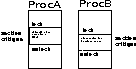
\includegraphics[width=300px]{fig32.pdf}\\

\titre{Utilisation :} Une \titre{Variable de condition} s'utilise toujours de paire avec un mutex. \\

\titre{3 primitives :}
\begin{enumerate}
	\item cond\_wait(C: Variable de condition, M:Mutex). Doit être appelé à l'intérieur d'une section critique protégée par M. Ce que ça fait :
	\begin{enumerate}	
		\item unlock(M)
		\item attendre un signal sur C
		\item lock(M)
	\end{enumerate}
	Intérêt de l'appel système pour faire ça : le passage de a à b est atomique, tout comme le passage entre b et c.
	\item cond\_signal(C: Variable de condition) Débloque au moins un processus bloqué sur C.
	\item cond\_broadcast(C: Variable de condition) Débloque tous les processus bloqués sur C.
\end{enumerate}

\titre{Remarque :} 
\begin{enumerate}
	\item Les variables de condition sont sans mémoire. Un signal émis lorsqu'aucun processus n'est en attente est perdu.
	\item Un cond\_wait s'exécute toujours à l'intérieur d'un tantque.
\end{enumerate} 

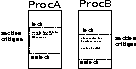
\includegraphics[width=300px]{fig33.pdf}\newpage

\titre{Producteurs/consommateurs :}\\
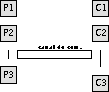
\includegraphics[width=200px]{fig34.pdf}\\
